\documentclass[a4paper,11pt]{article}

\usepackage[left=2cm, top=3cm, text={17cm, 24cm}]{geometry}
\usepackage[utf8]{inputenc}
\usepackage{times}
\usepackage[unicode]{hyperref}
\usepackage{fancyhdr}
\usepackage[fleqn]{amsmath}
\usepackage{amsfonts}
\usepackage{float}
\usepackage{graphicx}
\usepackage{gensymb}

\pagestyle{fancy}
\fancyhf{}
\rhead{Martin Kostelník, Marianne Jakonen, Ahmed Ansari\\\today}
\lhead{Advanced Data Analysis and Machine Learning \\ Intel Wireless Sensor Networks}

\begin{document}
	
	\section{Introduction}
	\label{section:intro}
		The dataset\footnote{Dataset publicly available at: \url{http://db.csail.mit.edu/labdata/labdata.html}} contains data collected from 54 sensors deployed in the Intel Berkeley Research lab. The collection period ranges from 28.2.2004 to 5.4.2004 and contains a total of roughly 2.3 million data samples. Each sensor collects data every 31 seconds and the data collected are: temperature, humidity, light and voltage. Each sensor also has a unique ID and stores the data with a timestamp and measurement ID.
	
	\section{Modelling goal}
	\label{section:goal}
		As per the assignment, the end goal is to use PCA to detect seasonality in the data. This will be done on both weekly and monthly basis. We will also study the correlation between the individual variables and create a dynamic model to predict future values for the most correlated variable. When we have this model, we can calculate how much ahead we can predict, it's window frame and the sampling frequency.
	
	\section{Data summary}
	\label{section:data}
		As described in section \ref{section:intro}, we have roughly 2.3 million data samples from 54 sensors placed at different location. The scheme of the data is shown in table \ref{table:scheme}.
		\begin{table}[H]
			\centering
			\begin{tabular}{|c|c|c|}
				\hline
				Name & Data type & Unit \\
				\hline
				Date & String & - \\
				\hline
				Time & String & - \\
				\hline
				Epoch & Int & - \\
				\hline
				Mote-id & Int & - \\
				\hline
				Temperature & Float & °C \\
				\hline
				Humidity & Float & \% \\
				\hline
				Light & Float & Lux \\
				\hline
				Voltage & Float & V\\
				\hline
			\end{tabular}
			\caption{Table showing column names, data types and units in the dataset.}
			\label{table:scheme}
		\end{table}
	
	When loading the dataset, we transform the \texttt{Date} and \texttt{Time} columns. We combine these into one column containing both using the correct datatype from pandas library.
	
	\subsection{Value ranges}
	\label{subsection:ranges}
		Now let's take a look at the value ranges of each column. We can find theoretical value ranges for some of the columns in the dataset documentation. There are no limits to the temperature column. We also find the actual value ranges present in the dataset for each column. These can be seen in \ref{table:ranges}. We can see that for some columns, there are non-sensical values that need to be removed and this also shows that there might be many outliers in the data.
		\begin{table}[H]
			\centering
			\begin{tabular}{|c|c|c||c|c|}
				\hline
				Name & Min\_T & Max\_T & Min\_R & Max\_R \\
				\hline
				Date & 28.2.2004 & 5.4.2004 & 28.2.2004 & 5.4.2004 \\
				\hline
				Time & 00:00 & 23:59 & 00:58:15 & 11:02:32 \\
				\hline
				Epoch & 0 & - & 0 & 65535\\
				\hline
				Mote-id & 1 & 54 & 1 & 65407 \\
				\hline
				Temperature & -273.15 & - & -38.4 & 385.568 \\
				\hline
				Humidity & 0 & 100 & -8983.13 & 137.512 \\
				\hline
				Light & 0 & - & 0 & 1847.36\\
				\hline
				Voltage & 2 & 3 & 0.009101 & 18.56 \\
				\hline
			\end{tabular}

			\caption{Table showing theoretical and actual value ranges in the dataset.}
			\label{table:ranges}
		\end{table}
	
	
	\subsection{Distribution}
	\label{subsection:distribution}
		There are four columns that contain numerical values. These are temperature, humidity, light and voltage. For now, we are only going to be interested in those columns. Figure \ref{figure:kde} shows kernel density estimation across the value ranges of each of these columns. Note that data were cleaned of outliers behind the theoretical ranges. Figure \ref{figure:box} uses boxplots to visualize the distribution. We can more clearly see where the mean sits and it seems to be around the usual values for all variables.
		\begin{figure}[H]
			\centering
			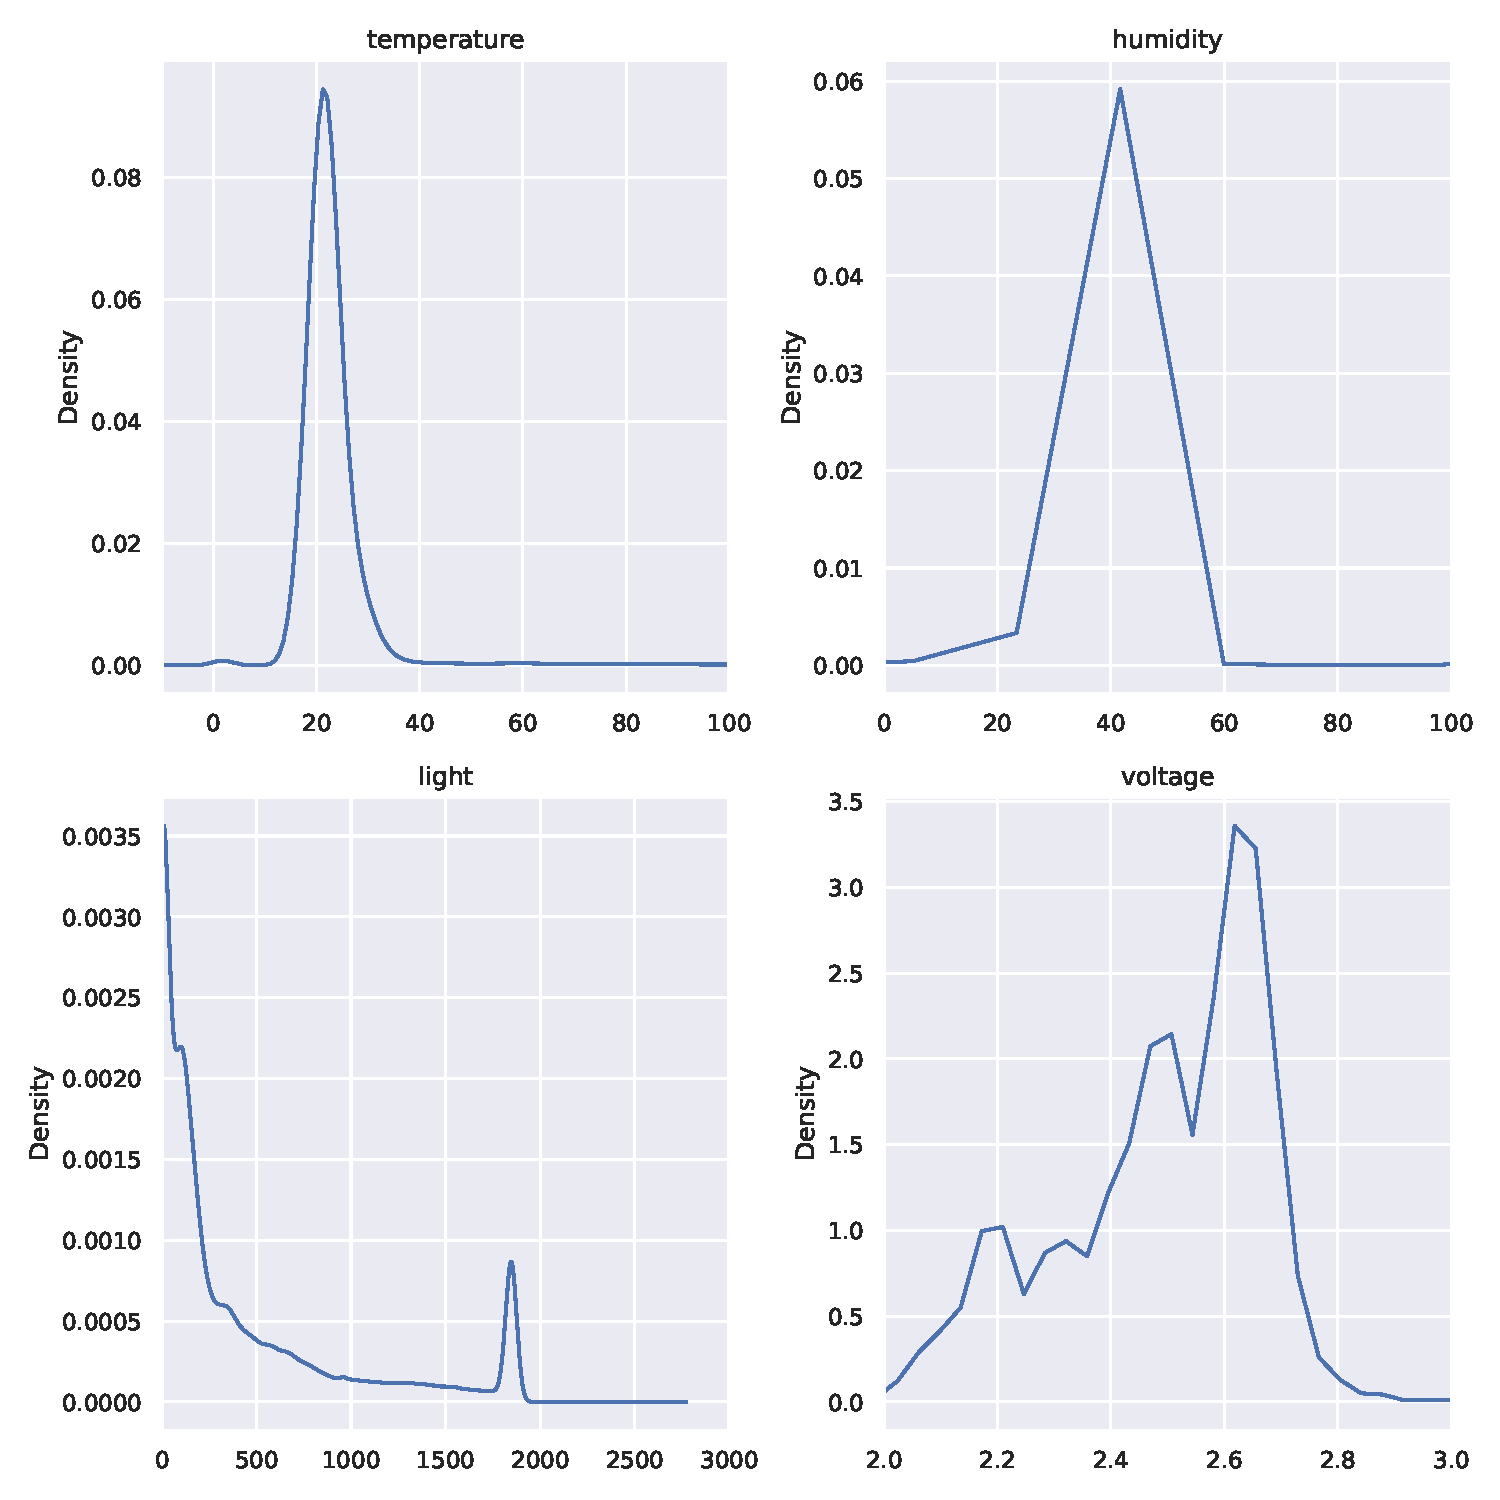
\includegraphics[scale=0.5]{density.pdf}
			\caption{Kernel density estimation for the numerical columns of the dataset.}
			\label{figure:kde}
		\end{figure}
		\begin{figure}[H]
			\centering
			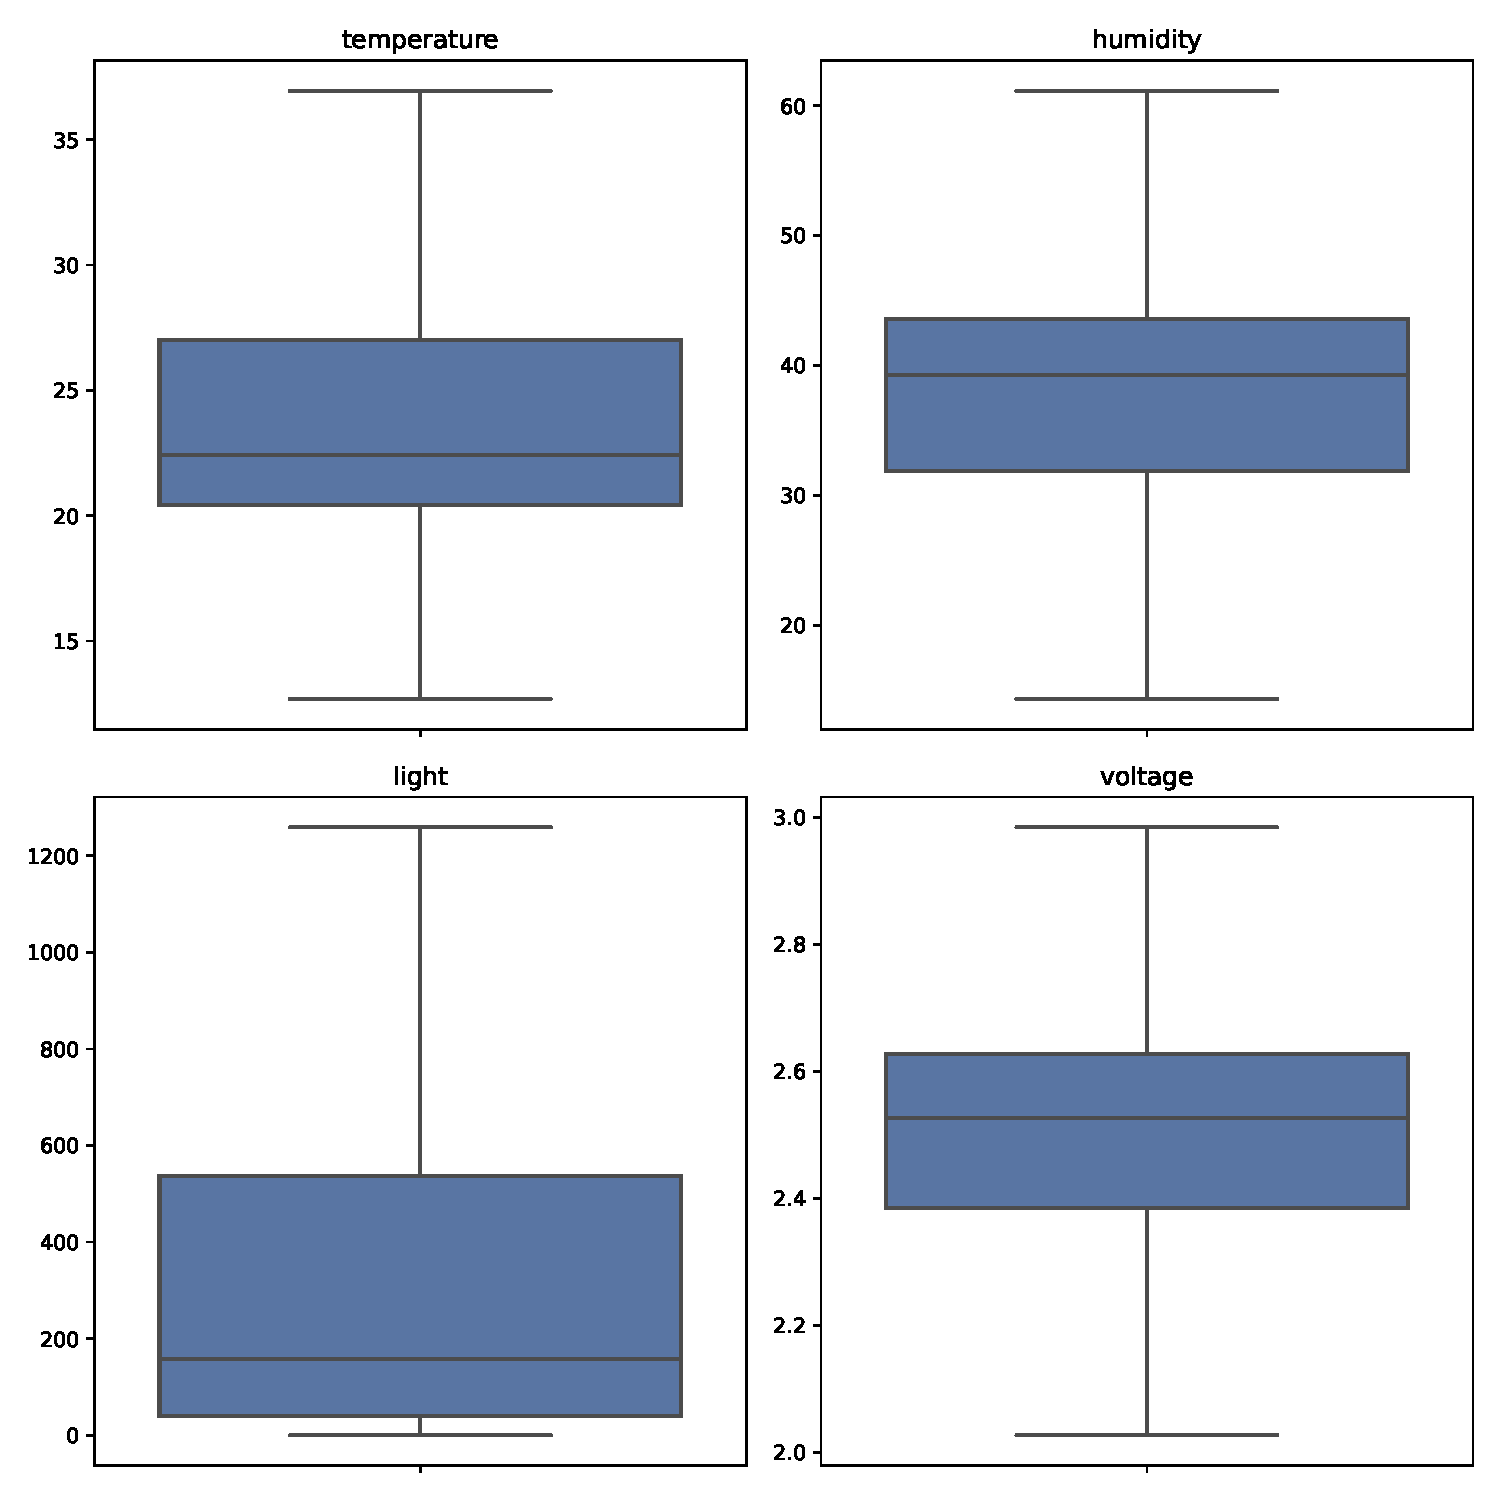
\includegraphics[scale=0.5]{boxplots.pdf}
			\caption{Data distribution visualized using boxplots.}
			\label{figure:box}
		\end{figure}
	
		The last figure, figure \ref{figure:timeseries} show the trend in the data over the measuring period. To create this figure, the dataset was averaged over 8 hour periods.  We can see a spike in temperature and change in the humidity at around the same time. Light amount seems to be changing based on the daily activity in the office. And lastly, as expected, the voltage in the batteries has a downward trend until the batteries are probably replaced.
		\begin{figure}[H]
			\centering
			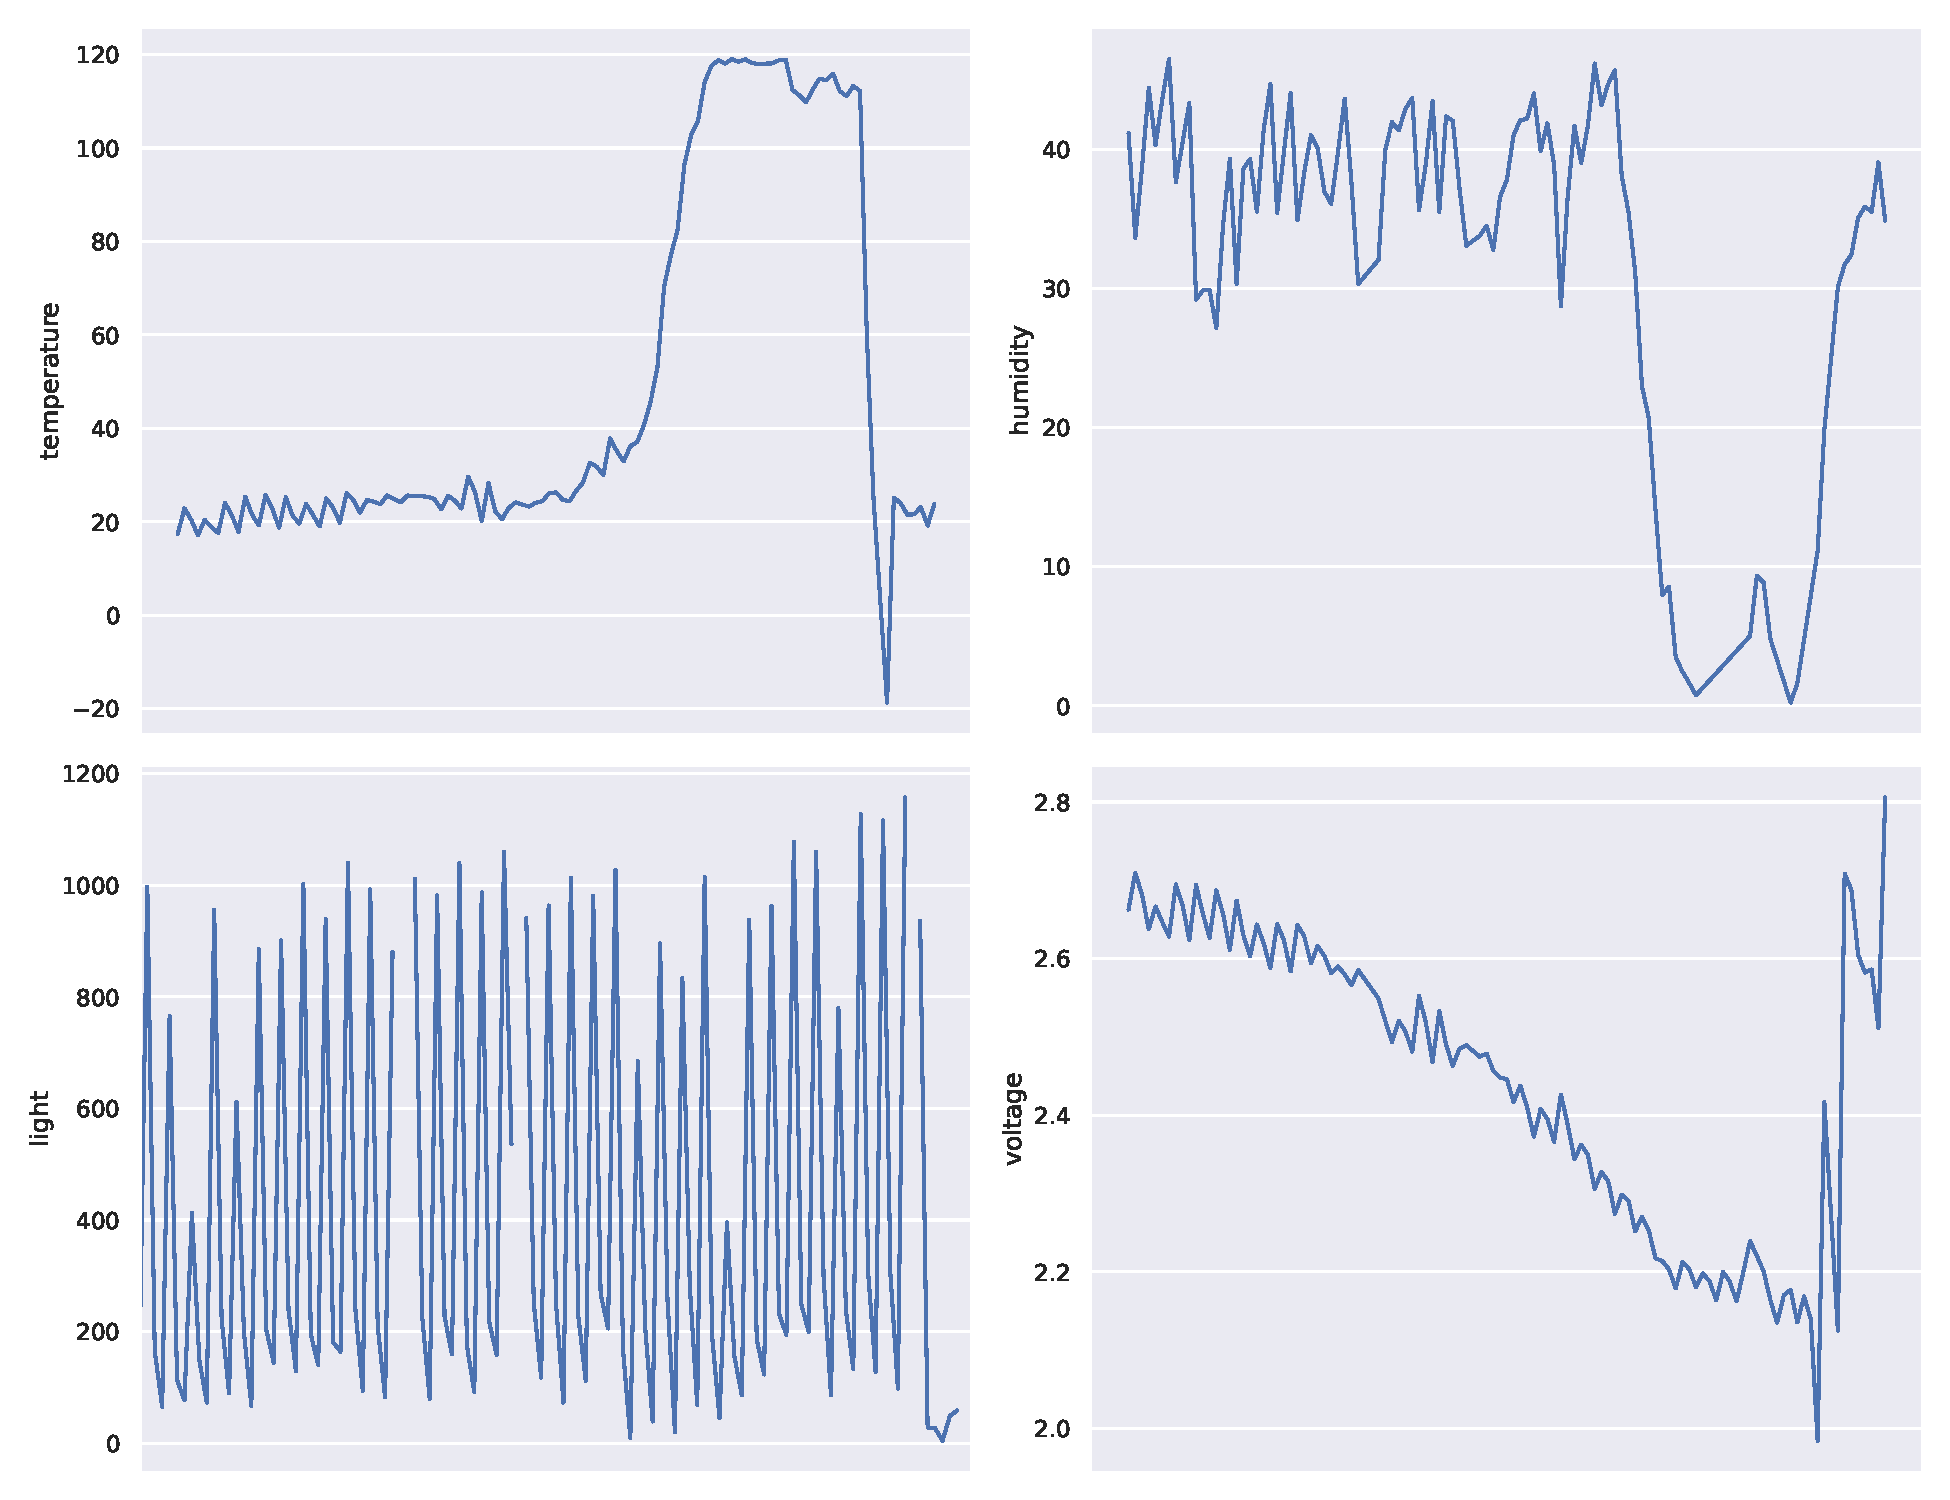
\includegraphics[scale=0.5]{timeseries.pdf}
			\caption{Time series of the data averaged over 8 hour time periods. Note that we only have light data for a shorter period of time than the other variables.}
			\label{figure:timeseries}
		\end{figure}
		
\end{document}
